\documentclass[14pt]{extreport}
\input{prop/preamble.inc}


\begin{document}

\SETgroup{K3121}
\SETstudent{Сакулин Иван}
\SETteacher{Курашова С.А.}
\SETdata{03.03.2025}
\SETnumber{1.02}
\SETtitle{Изучение скольжения тележки по наклонной плоскости}
\SETtitleT{}
\input{prop/title}

\noindent\textbf{1. Цель работы}

\begin{enumerate}[label=\arabic*)]
    \item Экспериментальная проверка равноускоренности движения
тележки по наклонной плоскости.
    \item Определение величины ускорения свободного падения $g$.
\end{enumerate}

\noindent\textbf{2. Задачи, решаемые при выполнении работы}

\begin{enumerate}[label=\arabic*)]
    \item Измерение времени движения тележки по рельсу с фиксированным углом наклона.
    \item Измерение времени движения тележки по рельсу при разных углах наклона рельса к горизонту.
    \item  Исследование движения тележки при фиксированном угле наклона рельса. Проверка равноускоренности движения тележки.
    \item  Исследование зависмости ускорения тележки от угла наклона рельса к горизонту. Определение ускорения свободного падения.
\end{enumerate}

\noindent\textbf{3. Объект исследования}

Равноускоренное движение тележки по рельсе.

\noindent\textbf{4. Метод экспериментального исследования}

Проведение измерений времени прохождения тележкой различных расстояний, получение экспериментальных данных, вычисление необходимых величин.

\noindent\textbf{5. Рабочие формулы и исходные данные}

Величины из теоретической зависимости $Y=aZ$:
\begin{equation*}
    Y=x_2 - x_1, \quad Z= \frac{t_2^2-t_1^2}{2}
\end{equation*}

Коэффициент $a$  из теоретической зависимости $Y=aZ$ и его среднеквадратическое отклонение (СКО) $\sigma_a$ (здесь $N = 5$):
\begin{equation*}
    a=\frac{\sum\limits^{N}_{i=1}Z_iY_i}{\sum\limits^{N}_{i=1}Z_i^2}, \quad 
    \sigma_a=\sqrt{\frac{\sum\limits^{N}_{i=1}(Y_i-aZ_i)^2}{(N-1)\sum\limits^{N}_{i=1}Z_i^2}}
\end{equation*}

Абсолютная погрешность ускорения (коэффициента $a$) для доверительной вероятности $\alpha = 0.90$, относительная погрешность:
\begin{equation*}
    \Delta_a=2\sigma_a, \quad \varepsilon_a=\frac{\Delta_a}{a}\cdot100\%
\end{equation*}

Cинуса угла наклона рельса к горизонту:
\begin{equation*}
    \sin{\alpha} = \frac{(h_0 - h) - (h_0' - h')}{x'-x}
\end{equation*}

Значение ускорения и его погрешность для каждой серии измерений:
\begin{equation*}
    \langle a \rangle = \frac{2(x_2 - x_1)}{{\langle t_2 \rangle}^2 - {\langle t_1 \rangle}^2}
\end{equation*}

\begin{equation*}
\Delta a = \langle a\rangle \sqrt{
    \frac{(\Delta x_{u2})^2 + (\Delta x_{u1})^2}{(x_2 - x_1)^2} + 
    4\frac{(\langle t_1\rangle \Delta t_1)^2 + (\langle t_2\rangle \Delta t_2)^2}{(\langle t_2\rangle^2 - \langle t_1\rangle^2)^2}
}
\end{equation*}

Коэффициенты линейной зависимости $a = A + B \sin{\alpha}$

\begin{equation*}
B \equiv g = \frac{
    \sum\limits_{i=1}^N a_i \sin\alpha_i - \frac{1}{N}\left(\sum\limits_{i=1}^N a_i\right)\left(\sum\limits_{i=1}^N \sin\alpha_i\right)
}{
    \sum\limits_{i=1}^N \sin^2\alpha_i - \frac{1}{N}\left(\sum\limits_{i=1}^N \sin\alpha_i\right)^2
}
\end{equation*}

\begin{equation*}
A = \frac{1}{N}\left(\sum_{i=1}^N a_i - B\sum_{i=1}^N \sin\alpha_i\right)
\end{equation*}

CКО для ускорение свободного падения (коэффициента $B$):

\begin{equation*}
\sigma_g = \sqrt{\frac{\sum_{i=1}^N d_i^2}{D(N-2)}},
\end{equation*}
\begin{equation*}
\text{где} \quad
d_i = a_i - (A + B \sin \alpha_i),
\quad
D = \sum_{i=1}^N \sin^2\alpha_i - \frac{1}{N} \left( \sum_{i=1}^N \sin\alpha_i \right)^2
\end{equation*}

\noindent\textbf{6. Измерительные приборы}

\begin{table}[H]
\centering
\small
\caption{Измерительные приборы}
\begin{tabular}{|l|c|c|c|}
\hline
\textbf{Наименование}         & \textbf{Предел измерений} & \textbf{Цена деления} & \({\Delta_u}\) \\ \hline
Линейка на рельсе             & 1,3\,м                    & 1\,см/дел             & 5\,мм             \\ \hline
Линейка на угольнике          & 250\,мм                   & 1\,мм/дел             & 0,5\,мм           \\ \hline
ПКЦ-3 в режиме секундомера    & 100\,с                    & 0,1\,с                & 0,1\,с            \\ \hline
\end{tabular}
\end{table}

\noindent\textbf{7. Схема установки} 
% ИЛИ Перечень схем, которые составляют Приложение 1.

\begin{figure}[H]
    \centering
    \includegraphics[width=1\linewidth]{1.02.physics-cheme.png}
    \caption{Схема установки}
    \label{picture:cheme}
\end{figure}

\newpage

\noindent\textbf{8. Результаты прямых измерений и их обработки} 
%(таблицы, примеры расчетов).

\begin{table}[H]
\centering
\caption{Фиксированные координаты (горизонтальное положение)}
\label{tab:table2}
\begin{tabular}{|c|c|c|c|}
\hline
\(x_1, \, \text{м}\) & \(x_2, \, \text{м}\) & \(h_0, \, \text{мм}\) & \(h_0', \, \text{мм}\) \\ \hline
$0.220 \pm 0.005$ & $1.000 \pm 0.005$ & $180.0 \pm 0.5$ & $181.0 \pm 0.5$ \\ \hline
\end{tabular}
\end{table}

\begin{table}[H]
\centering
\caption{Результаты прямых измерений (Задание 1)}
\label{tab:table3}
\begin{tabular}{|c|c|c|c|c|c|c|}
\hline
№ & \multicolumn{4}{c|}{Измеренные величины} & \multicolumn{2}{c|}{Рассчитанные величины} \\
\cline{2-7} 
& \(x_1, \, \text{м}\) & \(x_2, \, \text{м}\) & \(t_1, \, \text{c}\) & \(t_2, \, \text{c}\) & \(x_2 - x_1, \, \text{м}\) & \(\frac{t_2^2 - t_1^2}{2}, \, \text{c}^2\) \\ \hline
1 & 0.15 & 0.4 & 1.3 & 2.4 & $0.250 \pm 0.005$ & $3.73 \pm 0.18$ \\ \hline
2 & 0.15 & 0.5 & 1.2 & 2.7 & $0.350 \pm 0.005$ & $4.37 \pm 0.20$ \\ \hline
3 & 0.15 & 0.7 & 1.3 & 3.3 & $0.550 \pm 0.005$ & $6.29 \pm 0.24$ \\ \hline
4 & 0.15 & 0.9 & 1.2 & 3.7 & $0.750 \pm 0.005$ & $7.57 \pm 0.26$ \\ \hline
5 & 0.15 & 1.1 & 1.3 & 4.2 & $0.950 \pm 0.005$ & $9.67 \pm 0.29$ \\ \hline

\end{tabular}
\end{table}

Результаты прямых измерений задания 2 представлены в таблице \ref{tab:table5} в Приложении 1.

\noindent\textbf{9. Расчет результатов косвенных измерений} 
%(таблицы, примеры расчетов).

\textbf{Задание 1.}

По формулам были посчитаны $a = 0.093\text{м}/\text{c}^2$ и $\sigma_a \approx 0.00454$.
Затем погрешности $\delta_a = 0.009\text{м}/\text{c}^2$ и $\varepsilon_a = 10\%$ Результат:

\begin{equation*}
a = (0.093 \pm 0.009)\text{м}/\text{c}^2, \quad \varepsilon_a = 10\%, \quad \alpha=0.95
\end{equation*}

\textbf{Задание 2.}

\begin{table}[H]
\centering
\caption{Результаты расчетов (Задание 2)}
\label{tab:table4}
\begin{tabular}{|c|c|c|c|c|}
\hline
$N_{\text{ПЛ}}$ & $\sin \alpha$ & $\langle t_1 \rangle \pm \Delta t_1, \, \text{c}$ & $\langle t_2 \rangle \pm \Delta t_2, \, \text{c}$ & $\langle a \rangle \pm \Delta a, \, \frac{\text{м}}{\text{c}^2}$ \\
\hline
1 & 0.013 & $1.24 \pm 0.10$ & $4.20 \pm 0.07$ & $0.118 \pm 0.005$ \\ \hline
2 & 0.023 & $0.90 \pm 0.07$ & $3.00 \pm 0.07$ & $0.232 \pm 0.012$ \\ \hline
3 & 0.035 & $0.70 \pm 0.07$ & $2.42 \pm 0.09$ & $0.354 \pm 0.029$ \\ \hline
4 & 0.046 & $0.60 \pm 0.07$ & $2.10 \pm 0.07$ & $0.469 \pm 0.034$ \\ \hline
5 & 0.058 & $0.54 \pm 0.10$ & $1.90 \pm 0.07$ & $0.57 \pm 0.05$ \\ \hline

\end{tabular}
\end{table}

Пример расчетов для $N_{\text{ПЛ}}=1$:
\begin{equation*}
    \sin{\alpha} = \frac{(h_0 - h) - (h_0' - h')}{x'-x}
    =\frac{(0.18 - 0.229) - (0.181 - 0.185)}{1.00-0.22} \approx 0.013
\end{equation*}
\begin{equation*}
\langle t_1 \rangle = \frac{1}{N}\sum\limits_{i=1}^{N} t_{1_i} = 1.24c, \quad
\langle t_2 \rangle = \frac{1}{N}\sum\limits_{i=1}^{N} t_{2_i} = 4.20c
\end{equation*}
\begin{equation*}
    \langle a \rangle = \frac{2(x_2 - x_1)}{{\langle t_2 \rangle}^2 - {\langle t_1 \rangle}^2} = \frac{2\cdot(0.22 - 1.00)}{4.20^2 - 1.24^2} \approx 0.118 \text{м/с}^2
\end{equation*}

Найдём коэффициенты линейной зависимости $a = A + B \sin{\alpha}$

\begin{equation*}
B \equiv g = \frac{
    \sum\limits_{i=1}^N a_i \sin\alpha_i - \frac{1}{N}\left(\sum\limits_{i=1}^N a_i\right)\left(\sum\limits_{i=1}^N \sin\alpha_i\right)
}{
    \sum\limits_{i=1}^N \sin^2\alpha_i - \frac{1}{N}\left(\sum\limits_{i=1}^N \sin\alpha_i\right)^2
} \approx 
\end{equation*}
\begin{equation*}
A = \frac{1}{N}\left(\sum_{i=1}^N a_i - B\sum_{i=1}^N \sin\alpha_i\right) \approx 
\end{equation*}

По формулам были посчитаны $g_\text{эксп}$ его и погрешности:
\begin{equation*}
g_\text{эксп} = (10.2 \pm 0.5)\text{м}/\text{c}^2, \quad \varepsilon_a = 5\%, \quad \alpha=0.95
\end{equation*}

Сравним с $g_\text{табл} = 9.81908$:
\begin{equation*}
|g_\text{табл} - g_\text{эксп}| \approx 0.33\text{м}/\text{c}^2, \quad \varepsilon = \frac{|g_\text{табл} - g_\text{эксп}|}{g_\text{эксп}} = 3.3\%
\end{equation*}

\noindent\textbf{10. Расчет погрешностей измерений}
%(для прямых и косвенных измерений).

\textbf{Задание 1.}

Абсолютная погрешность для $Y=x_2-x_1$ (при $\Delta_{x_1}=\Delta_{x_2}=\frac{2}{3}\Delta_{x\text{и}} = 0.005м$): 
{\fontsize{13}{13}\selectfont\begin{equation*}
    \Delta_Y =
    \sqrt{(\frac{\partial Y}{\partial x_1}\Delta_{x_1})^2+(\frac{\partial Y}{\partial x_2}\Delta_{x_2})^2} =
    \sqrt{(-\frac{2}{3}\Delta_{x\text{и}})^2+(\frac{2}{3}\Delta_{x\text{и}})^2} = 
    \frac{2\sqrt{2}}{3}\Delta_{x\text{и}} \approx 0.005\text{м}
\end{equation*}}

Относительные погрешности $\varepsilon_Y=\frac{\Delta_Y}{Y}\cdot100\%$:

$\varepsilon_{Y_1}=1.9\%$, $\varepsilon_{Y_2}=1.3\%$, $\varepsilon_{Y_3}=0.9\%$, $\varepsilon_{Y_4}=0.6\%$, $\varepsilon_{Y_5}=0.5\%$.

Абсолютные погрешности для $Z= \frac{t_2^2-t_1^2}{2}$  ($\Delta_{t_1}=\Delta_{t_2}=\frac{2}{3}\Delta_{t\text{и}} = 0.1c$): 

{\fontsize{13}{13}\selectfont\begin{equation*}
    \Delta_Z =
    \sqrt{(\frac{\partial Z}{\partial t_1}\Delta_{t_1})^2+(\frac{\partial Z}{\partial t_2}\Delta_{t_2})^2} =
    \sqrt{(t_1\Delta_{t_1})^2+(t_1\Delta_{t_2})^2} =
    \frac{2}{3}\Delta_{t\text{и}}\sqrt{t_1^2+t_1^2}
\end{equation*}}

$\Delta_{Z_1}=0.18 {c^2}$, $\Delta_{Z_2}=0.20 {c^2}$, $\Delta_{Z_3}=0.24 {c^2}$, $\Delta_{Z_4}=0.26 {c^2}$, $\Delta_{Z_5}=0.29 {c^2}$.

Относительные погрешности $\varepsilon_Z=\frac{\Delta_Z}{Z}\cdot100\%$:

$\varepsilon_{Z_1}=5\%$, $\varepsilon_{Z_2}=5\%$, $\varepsilon_{Z_3}=3.8\%$, $\varepsilon_{Z_4}=3.4\%$, $\varepsilon_{Z_5}=3.0\%$.

\textbf{Задание 2.}

Пример рассчета погрешности для ${\langle t_{1_1} \rangle}$:
\begin{equation*}
    \sigma_{\langle t_{1_1} \rangle}=\sqrt{\frac{\sum\limits_{i=1}^{n}(x_i - {\langle t_{1_1} \rangle})^2}{n(n-1)}} \approx 0.0245, \quad
    \Delta_{\langle t_{1_1} \rangle}=t_{\alpha, n}\sigma_{\langle t_{1_1} \rangle} = 2.78 \cdot 0.0245 \approx 0.0681c
\end{equation*}
\begin{equation*}
    \Delta_{t_{1_1}}=\sqrt{\Delta_{\langle {t_{1_1}} \rangle}^2+(\frac{2}{3}\Delta_{\text{и}t})^2} = 0.10c, \quad \varepsilon_{t_{1_1}}=\frac{\Delta_{t_{1_1}}}{{t_{1_1}}}\cdot100\% = 8\%
\end{equation*}

Рассчёт абсолютных погрешностей ускорений: $\Delta_{a_1} = 0.005\text{м}/\text{c}^2$, 

$\Delta_{a_2} = 0.012\text{м}/\text{c}^2$, $\Delta_{a_3} = 0.029\text{м}/\text{c}^2$, $\Delta_{a_4} = 0.034\text{м}/\text{c}^2$, $\Delta_{a_5} = 0.05\text{м}/\text{c}^2$

Рассчитал относительные погрешности ускорений:

$\varepsilon_{a_1} = 3.8\%$, $\varepsilon_{a_2} = 5\%$, $\varepsilon_{a_3} = 8\%$, $\varepsilon_{a_4} = 7\%$, $\varepsilon_{a_5} = 8\%$

Рассчитал СКО для ускорения свободного падения:

$d_1 \approx -0.0073$, $d_2 \approx 0.0026$, $d_3 \approx 0.0075$, $d_4 \approx 0.0054$, $d_5 \approx -0.0083$

$D \approx 0.0013$

$\sigma_{g_\text{эксп}} \approx 0.2367$

Посчитал погрешности ускорения свободного падения:

\begin{equation*}
\Delta_{g_\text{эксп}} = 2*\sigma_{g_\text{эксп}} = 0.5, \quad \varepsilon_{g_\text{эксп}}=\frac{\Delta_{g_\text{эксп}}}{g_\text{эксп}}\cdot100\% = 5\%
\end{equation*}

\noindent\textbf{11. Графики }
% ИЛИ Перечень графиков, которые составляют Приложение 2.

Перечень графиков в Приложении 2: 
\begin{itemize}
    \item график зависимости $Y(Z)$ -- рисунок \ref{fig:graphic1},
    \item график зависимости $a(\sin\alpha)$ -- рисунок \ref{fig:graphic2}.
\end{itemize}

\newpage
\noindent\textbf{12. Окончательные результаты}

Доверительный интервала для ускорения (1 задание):
\begin{equation*}
a = (0.093 \pm 0.009)\text{м}/\text{c}^2, \quad \varepsilon_a = 10\%, \quad \alpha=0.95
\end{equation*}

Значение ускорения свободного падения, полученного экспериментально:
\begin{equation*}
g_\text{эксп} = (10.2 \pm 0.5)\text{м}/\text{c}^2, \quad \varepsilon_a = 5\%, \quad \alpha=0.95
\end{equation*}

Абсолютное и относительное отклонение измеренного ускорения свободного падения от его табличного значения $g_\text{табл} = 9.81908$:
\begin{equation*}
|g_\text{табл} - g_\text{эксп}| \approx 0.33\text{м}/\text{c}^2, \quad \varepsilon = \frac{|g_\text{табл} - g_\text{эксп}|}{g_\text{эксп}} = 3.3\%
\end{equation*}

\noindent\textbf{13. Выводы и анализ результатов работы}

В ходе работы были исследованы равноускоренное движение тележки по наклонной плоскости и определено ускорение свободного падения $g$.

Линейный характер графика $Y(Z)$ подтверждает равноускоренное движение. График $a(\sin\alpha)$ также демонстрирует линейную зависимость, что согласуется с теорией $a=g\sin\alpha$. Небольшой разброс точек на графике $a(\sin\alpha)$ связан с накоплением погрешностей при увеличении угла наклона.

Эталонное значение $g_\text{табл}$ входит в доверительный интервал измеренного значения $g_\text{эксп}$ и относительное расхождение всего $3.3\%$ - это указывает на корректность методики измерений.

Отрицательные значения $\sin\alpha$ оправдываются измерениями высот $h$ и $h'$ с другой стороны.

\newpage
\textbf{Контрольные вопросы}

1. \textbf{Перемещение} — это \textit{векторная величина}, соединяющий начальное положение тела с его конечным положением. \textbf{Траектория} — это \textit{геометрическая линия}, по которой движется тело. \textbf{Путь} — это \textit{скалярная величина}, длина траектории, которую проходит тело при движении.

2. Графики прямолинейного движения.
\begin{figure}[H]
    \centering
    \includegraphics[width=1\linewidth]{graphics/1.02.cq2.png}
    \label{fig:enter-label}
\end{figure}

3. Ускорение $a = 0$.

4. Модуль ускорения будет больше в \textbf{первом} случае, когда начальная скорость направлена вверх. При равной силе $mg\sin\alpha$, направленной вдоль вниз: в первом случае сила трения $\mu mg\cos\alpha$ будет направлена против направления движения вниз ($a = g\sin\alpha + \mu g\cos\alpha$), во втором - вверх ($a = g\sin\alpha - \mu g\cos\alpha$). 

5. Получение формулы для $\sin\alpha$.
\begin{figure}[H]
    \centering
    \includegraphics[width=0.7\linewidth]{graphics/1.02.cq5.png}
    \label{fig:enter-label}
\end{figure}

6. Так как в условиях задачи $F_\text{тр} = \mu mg\cos\alpha$, то при увеличении угла, сила уменьшается.
\begin{figure}[H]
    \centering
    \includegraphics[width=0.7\linewidth]{graphics/1.02.cq6.png}
    \label{fig:enter-label}
\end{figure}

7. Почти везде ускорение свободного падения \textbf{на экваторе ниже, чем на полюсах}, за счёт центробежных сил, возникающих при вращении планеты, а также потому, что радиус на полюсах меньше, чем на экваторе из-за сплюснутой формы планеты.

\newpage
\textbf{Приложение 1}

\begin{table}[H]
\centering
\caption{Результаты прямых измерений (Задание 2)}
\label{tab:table5}
\begin{tabular}{|>{\centering\arraybackslash}p{10mm}|>{\centering\arraybackslash}p{30mm}|>{\centering\arraybackslash}p{30mm}|>{\centering\arraybackslash}p{10mm}|>{\centering\arraybackslash}p{30mm}|>{\centering\arraybackslash}p{30mm}|}
\hline
$ N_{\text{ПЛ}} $ & $ h, \, \text{мм} $ & $ h', \, \text{мм} $ & № &  $t_1, \, \text{c}$ & $t_2, \, \text{c}$ \\
\hline
\multirow{5}{*}{1} & \multirow{5}{*}{191} & \multirow{5}{*}{182} & 1 & 1.2 & 4.2 \\ \cline{4-6}
& & & 2 & 1.2 & 4.2 \\ \cline{4-6}
& & & 3 & 1.2 & 4.2 \\ \cline{4-6}
& & & 4 & 1.3 & 4.2 \\ \cline{4-6}
& & & 5 & 1.3 & 4.2 \\ \hline
\multirow{5}{*}{2} & \multirow{5}{*}{200} & \multirow{5}{*}{183} & 1 & 0.9 & 3.0 \\ \cline{4-6}
& & & 2 & 0.9 & 3.0 \\ \cline{4-6}
& & & 3 & 0.9 & 3.0 \\ \cline{4-6}
& & & 4 & 0.9 & 3.0 \\ \cline{4-6}
& & & 5 & 0.9 & 3.0 \\ \hline
\multirow{5}{*}{3} & \multirow{5}{*}{210} & \multirow{5}{*}{184} & 1 & 0.7 & 2.4 \\ \cline{4-6}
& & & 2 & 0.7 & 2.4 \\ \cline{4-6}
& & & 3 & 0.7 & 2.4 \\ \cline{4-6}
& & & 4 & 0.7 & 2.4 \\ \cline{4-6}
& & & 5 & 0.7 & 2.5 \\ \hline
\multirow{5}{*}{4} & \multirow{5}{*}{219} & \multirow{5}{*}{184} & 1 & 0.6 & 2.1 \\ \cline{4-6}
& & & 2 & 0.6 & 2.1 \\ \cline{4-6}
& & & 3 & 0.6 & 2.1 \\ \cline{4-6}
& & & 4 & 0.6 & 2.1 \\ \cline{4-6}
& & & 5 & 0.6 & 2.1 \\ \hline
\multirow{5}{*}{5} & \multirow{5}{*}{229} & \multirow{5}{*}{185} & 1 & 0.5 & 1.9 \\ \cline{4-6}
& & & 2 & 0.5 & 1.9 \\ \cline{4-6}
& & & 3 & 0.6 & 1.9 \\ \cline{4-6}
& & & 4 & 0.6 & 1.9 \\ \cline{4-6}
& & & 5 & 0.5 & 1.9 \\ \hline

\multicolumn{6}{|l|}{$ N_{\text{ПЛ}} $ -- количество пластин} \\
\multicolumn{6}{|l|}{$ h $ -- высота на координате $x = 0,22 м$} \\
\multicolumn{6}{|l|}{$ h'$ -- высота на координате $x' = 1,00 м$} \\ \hline
\end{tabular}
\end{table}

\newpage
\textbf{Приложение 2}

\begin{figure}[H]
    \centering
    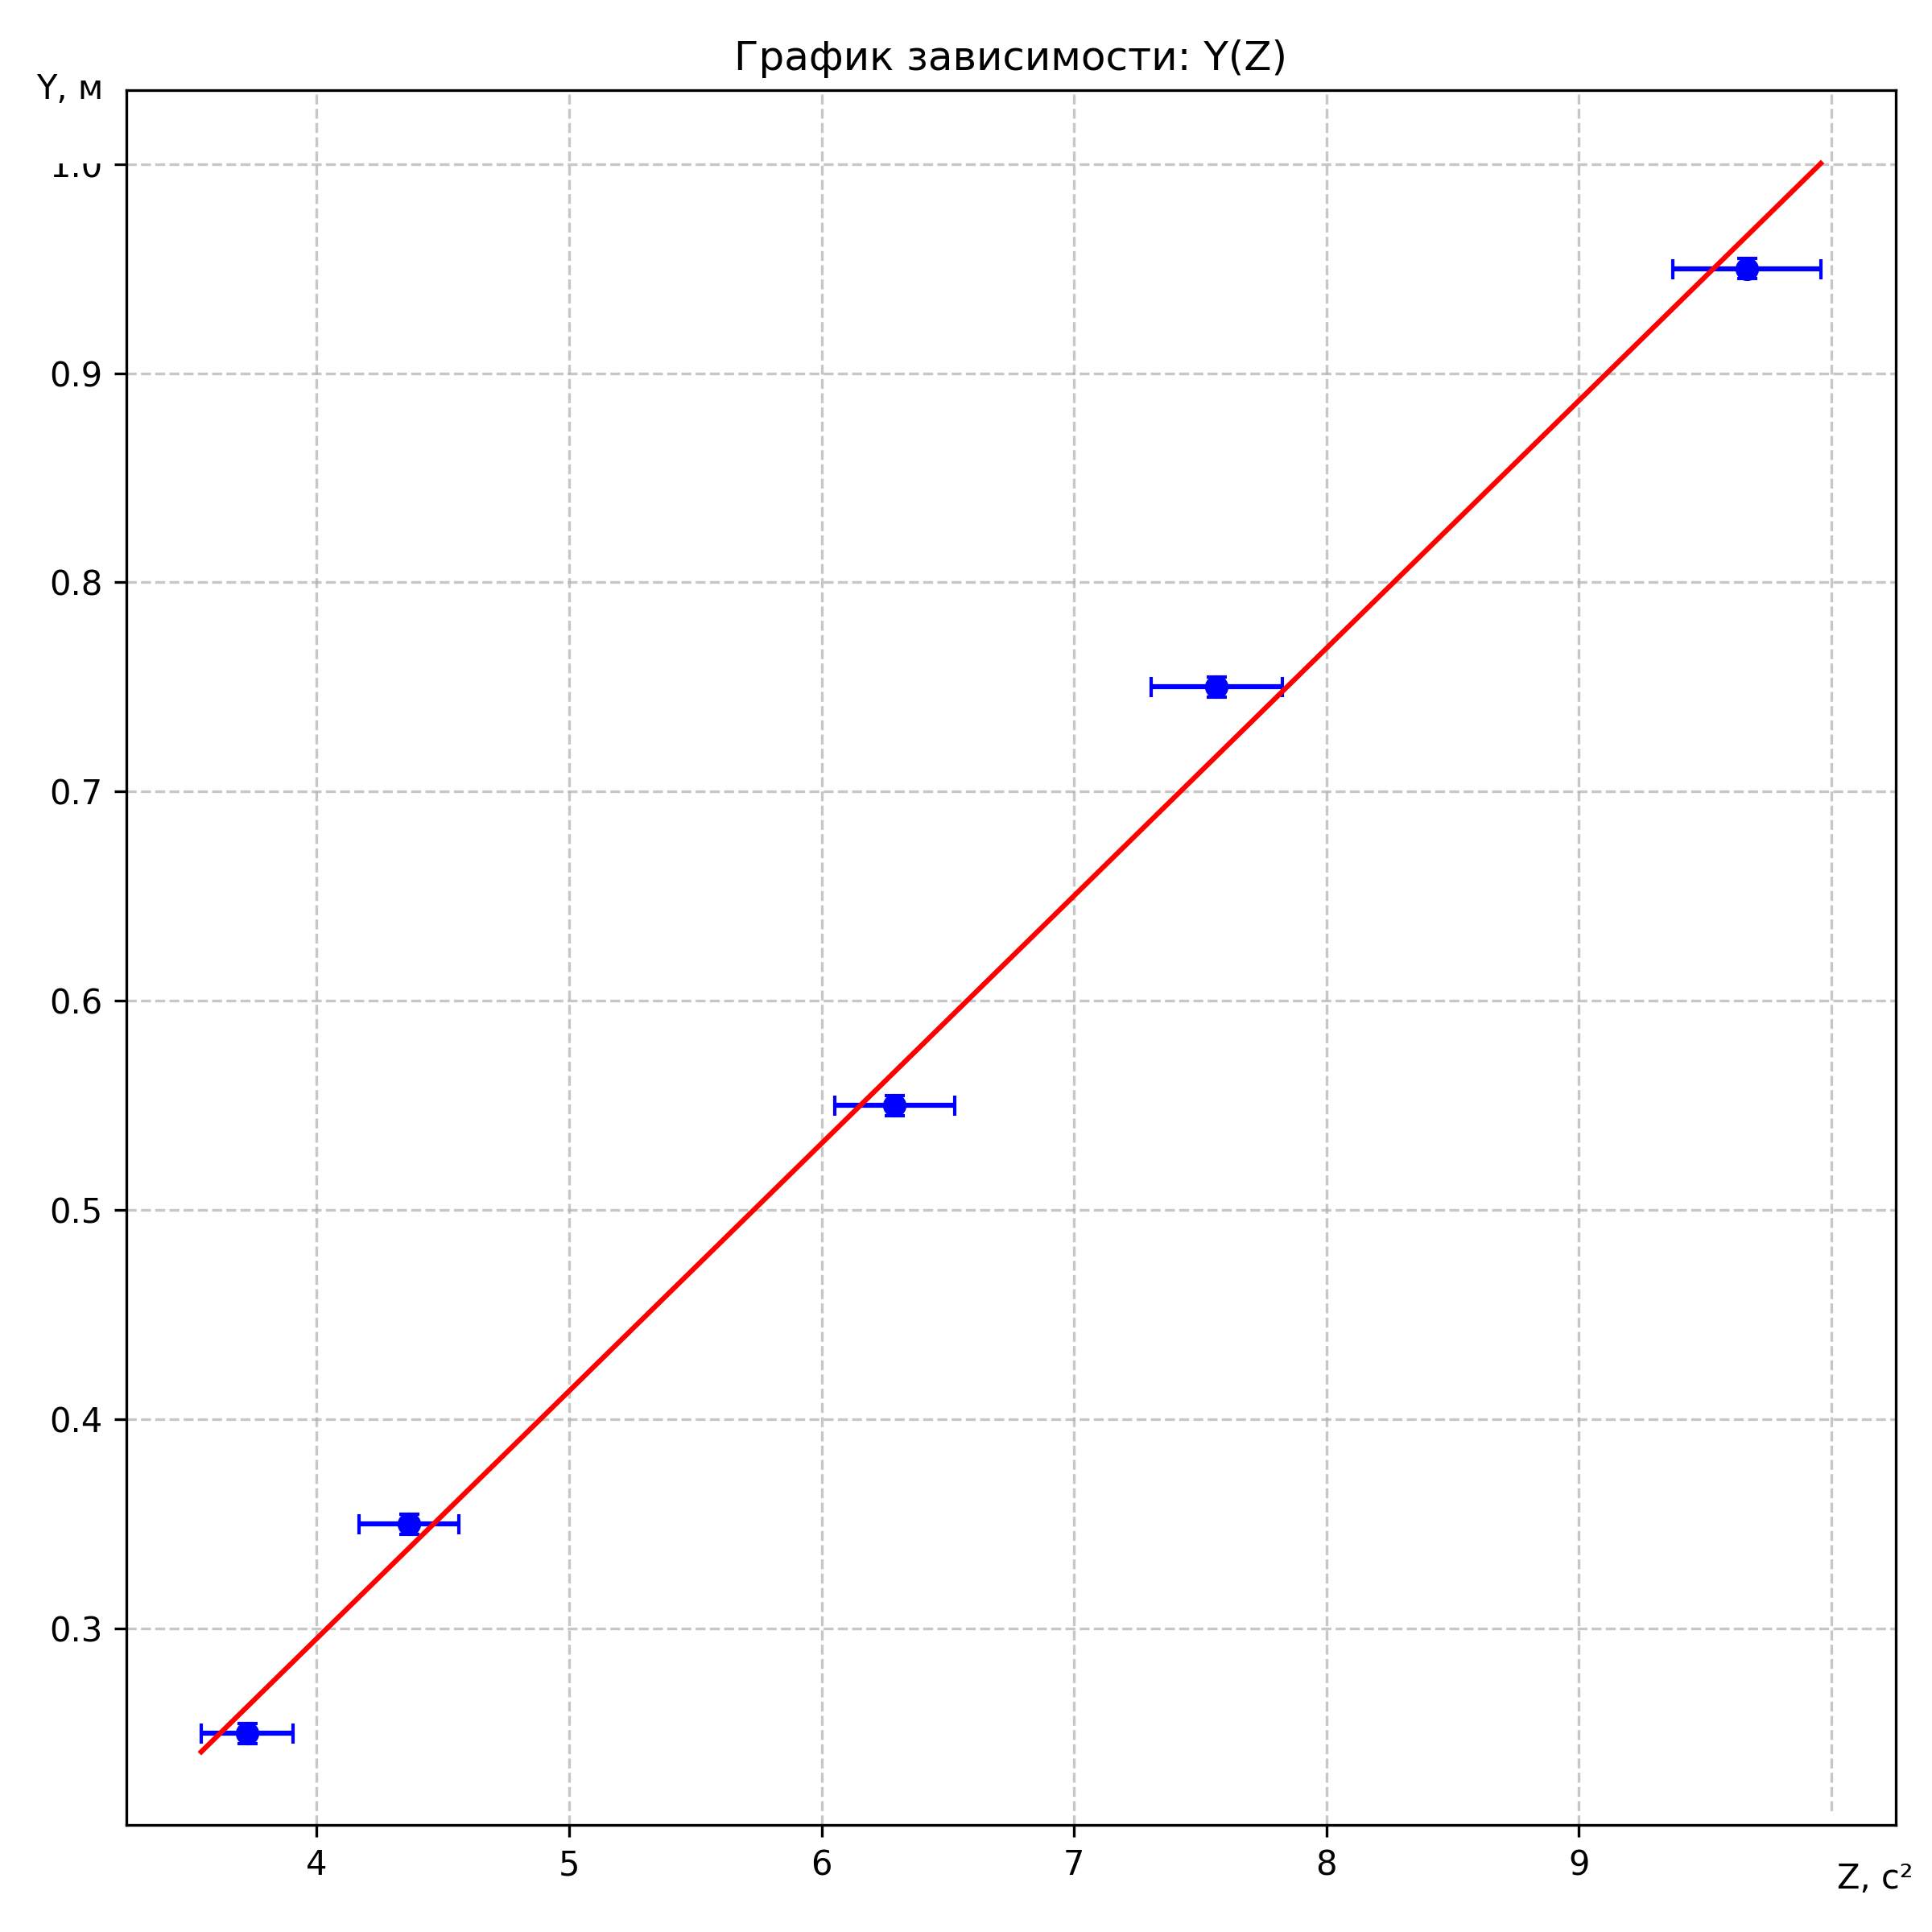
\includegraphics[width=1\linewidth]{1.02.g1.png}
    \caption{График зависимости $Y(Z)$}
    \label{fig:graphic1}
\end{figure}

\begin{figure}[H]
    \centering
    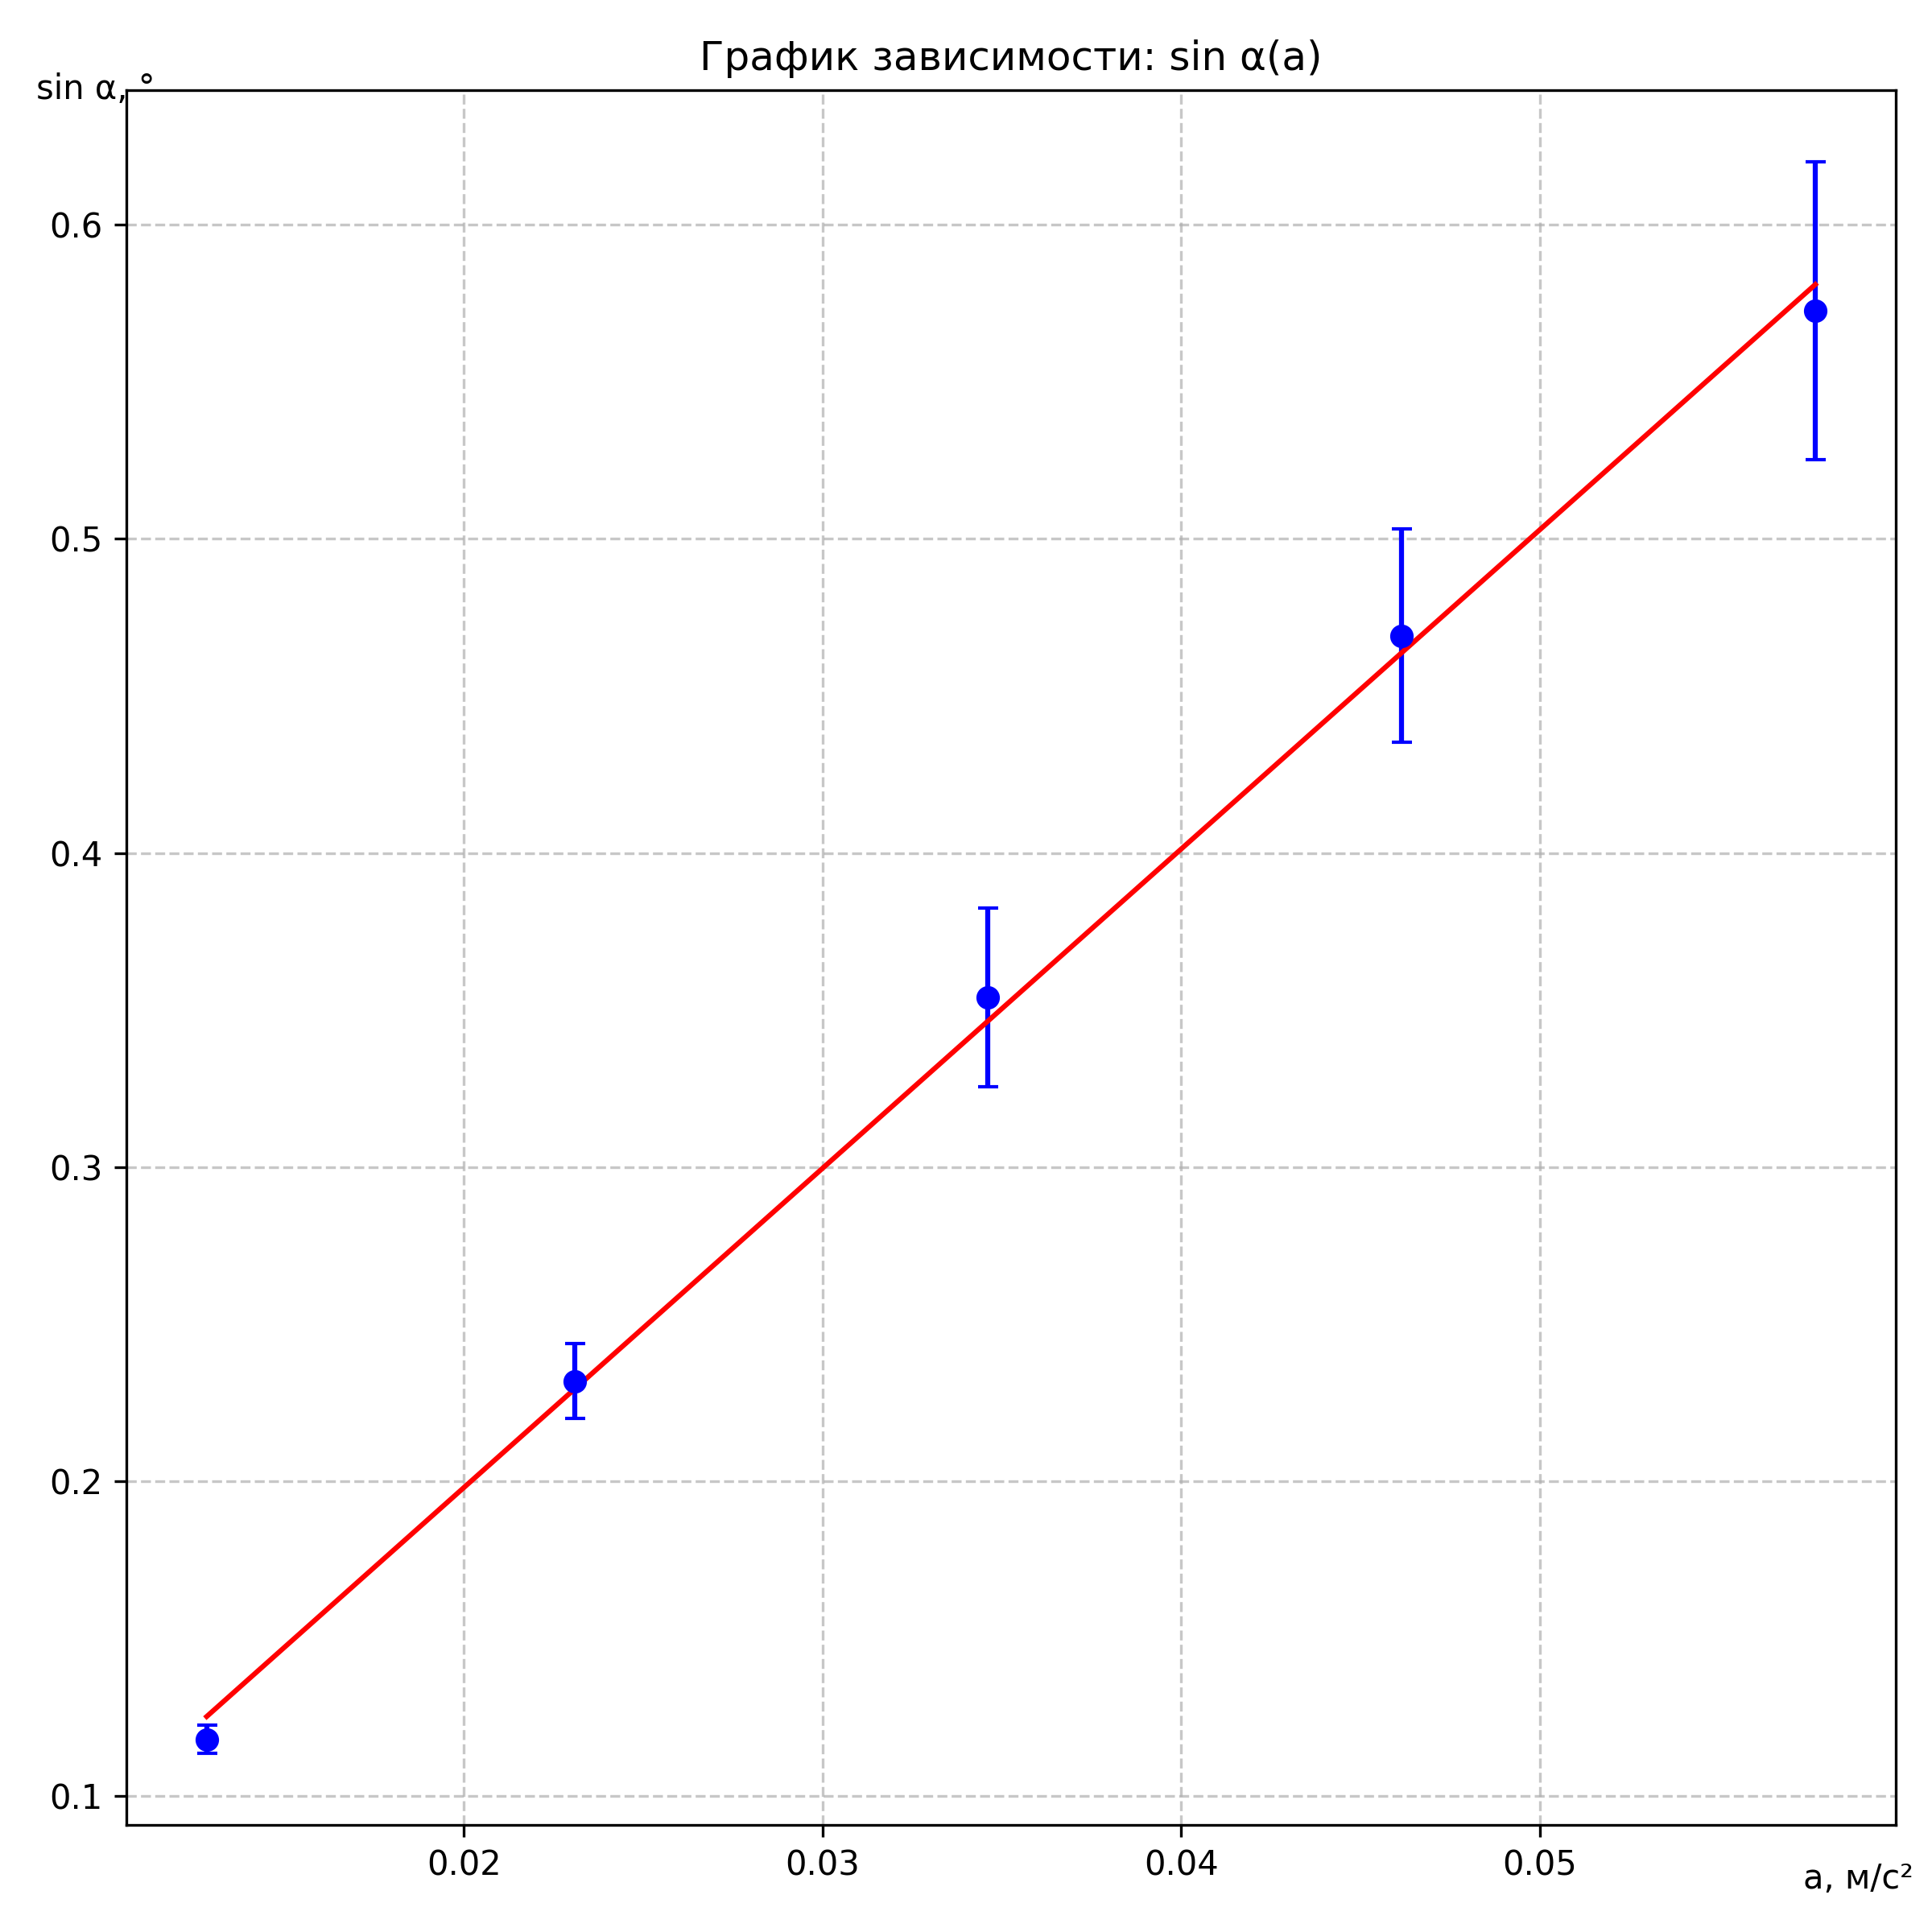
\includegraphics[width=1\linewidth]{1.02.g2.png}
    \caption{График зависимости $a(\sin\alpha)$}
    \label{fig:graphic2}
\end{figure}

\end{document}